\chapter{Introduction}
\addcontentsline{toc}{chapter}{Introduction}

	Capturing visual information of any kind have never been easier. Almost everyone of us posses a camera, be it a professional dSLR or a tiny one embedded into one of the ubiquitous smartphones. As human beings we have no difficulty understanding this data, just as we have no difficulty understanding what our eyes see. Unfortunately, the situation of our computers is the very opposite. Storage capacity of modern-day computers is overwhelming.  But even if hard-drives are full of images it is impossible to identify their semantic meaning without the aid of specialised algorithms, however. These algorithms often balance on the verge of image processing and machine learning --- they are a part of an area called computer vision. As Forsyth and Ponce \cite{ponce2011cv} have it: \begin{quote} computer vision is (...) an enterprise that uses statistical methods to disentangle data using models constructed with the aid of geometry, physics, and learning theory.\end{quote} The area of computer vision is not new. The original applications were industrial inspection or mobile robot navigation. More recent approaches consider problems such as human-machine interfaces, medical diagnostics, or image retrieval.
	
	How about semantic classification of scenes or objects? Suppose a mobile robot would know, or understand, what does it have to deal with. Suppose a robot would know that it is about to take, say, a glass of water. How would it affect the robot's behaviour? Could it have any impact on the force of the grip? or the speed and the manner of the planned object movement? Answers for all this questions are yes. Semantic classification is possible, but it requires clever mechanisms of computer vision and powerful computers. It can be seen as a part of a more general classification problem, which machine learning handles quite well. Suitable algorithms include, but are not limited to, artificial neural networks, deep belief networks, logistic regression, support vector machines and approaches based on probabilistic graphical models. One has to bear in mind that none of them can handle the problem directly. That is, it is inconceivable to feed a whole image as is into a classifier --- some degree of preprocessing is required. One such preprocessing technique is translation of image into a feature vector. What should this vector comprise of? A Bag of Words model is one technique that answers this question. This model has been first used for scene classification in 2004 in \cite{csurka2004visual} and maintains its popularity ever since.
	
	In this paper a technique for semantic object classification based on three dimensional point clouds is presented. The rest of this chapter is organised as follows: Section 1 describes the Bag of Words technique in detail. Construction of an image's model is discussed and the most popular algorithms are summarised. Section 2 provides basic information on the problem of classification, introduces basic concepts and methods of classification. Section 3 names C++ computer vision and general purpose libraries used in this project. Finally in Section 4 two datasets of RGBD images are outlined. The following chapters are titled ``Design'' and ``Experiments and Results''. The former contains description of required functionality of a programme for BoW object classification, its design and implementation details. The latter addresses topics of experimental setup, performed experiments and a summary of results. 
	
\section{Bow of Words}

	The Bag of Words (BoW) model is a an intermediate representation used in natural language processing, information retrieval and data mining [need pub]. The model can be seen as a simplification, for it obliterates any grammatical information and even word order contained within an original text document. What is left is an unstructured group of words, usually in a form of a vector or a histogram of word incidence.

	\begin{figure}[!ht]
	\centering
	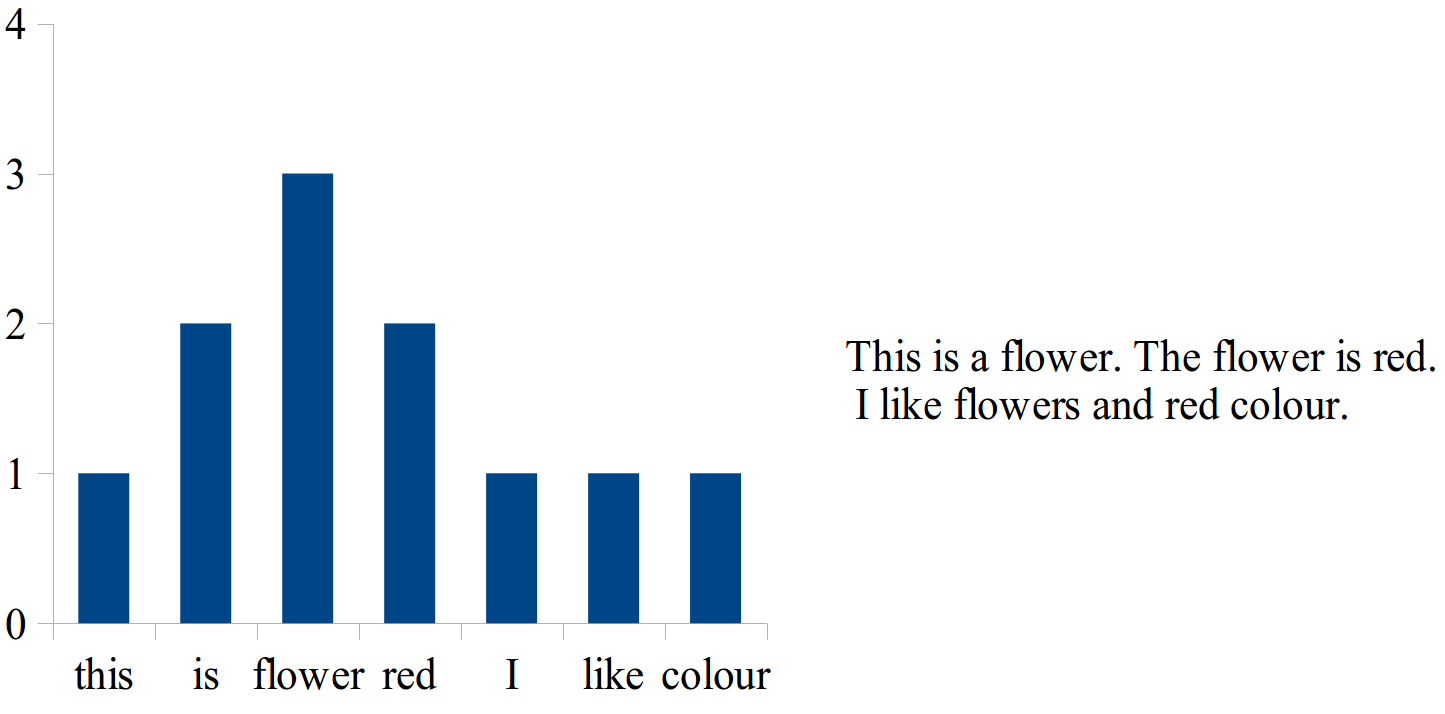
\includegraphics[width=0.7\textwidth]{figs/bow_example}
	\caption{Bag of Words histogram}
	\label{fig:bow_example}
	\end{figure}
	
	The figure \ref{fig:bow_example} shows a piece of text and its BoW model, where articles and punctuation marks were left out. In order to compare different documents a global dictionary must be built. The dictionary (codebook) is constructed by taking every word from all available documents and removing duplicates. One can image that if a dictionary is of any considerable size resulting representation of especially small documents will be very sparse.

	In natural language processing BoW representation is used to infer semantic meaning of documents [need pub]. If an image could be translated into a text document it might be possible to employ similar methods. A question arises: How does one make a text document from an image?

	\subsection{Processing Pipeline}	
	Tsai describes a well established pipeline that allows translation of images into text documents or BoW models \cite{tsai2012bag}. It consists of the following steps: (1) region detection, (2) feature extraction, (3) vector quantization and (4) BoW histogram formation as can be seen in the figure \ref{fig:bow_pipeline}. The author summarises the most commonly used methods for performing these tasks. 
	
	\begin{figure}[!ht]
	\centering
	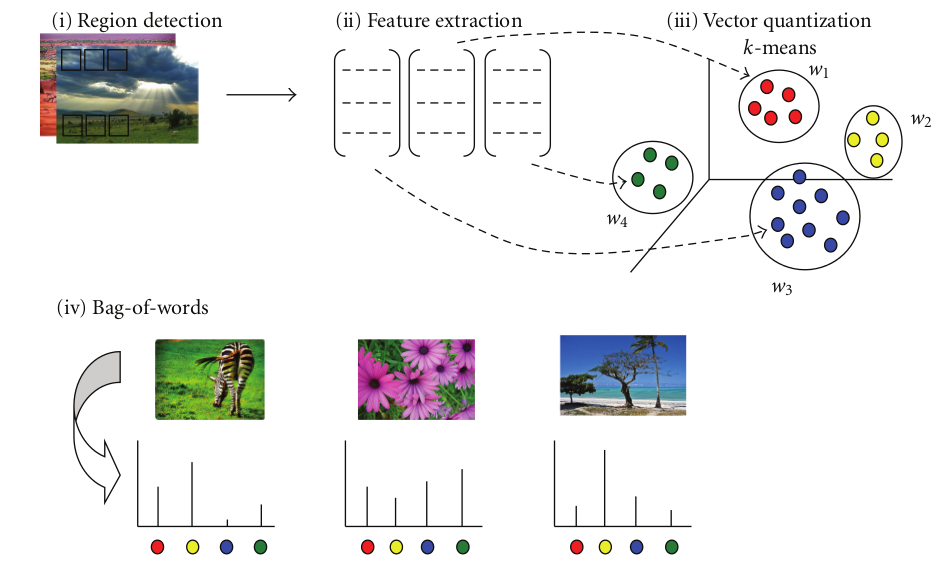
\includegraphics[width=0.75\textwidth]{figs/tsai2012}
	\caption{Bag of Words pipeline. The figure comes from \cite{tsai2012bag}}
	\label{fig:bow_pipeline}
	\end{figure}
	
		\subsubsection{Region Detection}
		Characteristic region detection is the first step in any Bag of Words framework. Numerous detection methods have been developed, but choosing the right one for any particular case might prove tricky. A good overview of various mechanisms is available in \cite{tsai2012bag}.
		
		The most common detectors make use of a Harris corner detector or image's first or second derivatives. A Harris-Laplace detector is an example of a Harris-based detector. The Harris function is scale adapted and its outcome is a subject to a Laplacian-of-Gaussian (LoG) operator, which selects relevant points in scale space. Images' regions' 2\textsuperscript{nd} derivatives, namely the regions' Hessians, can be combined with a LoG operator as well. This combination allows selection of points significant in the two spaces: the scale space and the Hessian's determinant space. The latter entails the speed at which pixel intensities change in the neighbourhood of a point.	
	
		A number of more complicated recipes for salient region localisation have been developed and implemented. These include for example SIFT \cite{sift_keypoint}, SUSAN \cite{susan_keypoint} and Intrinistic Shape Signatures \cite{iss_keypoint}. The majority of keypoint detection formulas is being developed for the 2D domain. A number of them have been adapted to 3D, however. A comparative evaluation of detection algorithms available in the PointCloud Library (PCL, discussed below) can be find in \cite{pcl_keypoint_comparision}. Another comprehensive study is \cite{3d_keypoint_eval}. All these formulas, called sparse feature detectors, resort to selection of maxima in specific state spaces. An entirely different scheme is to use a dense feature detector. That is, take a uniformly sampled grid of points. Dense detectors, unlike the sparse ones, take points from slow changing regions such as clear sky and calm ocean water. Li \emph{et al} showed that dense detectors generally outperform the sparse ones \cite{fei2005bayesian}.
		
		\subsubsection{Feature Extraction}
		Suppose only coordinates of a keypoint were found. In case of even smallest rotation or translation they would change and the keypoint would be lost. Keypoints should be described in a way that makes them invariant to affine transforms, changes in light intensity or colour saturation. All these properties are hard to achieve, but methods that meet some of the criteria exist.
		
		Keypoint description is usually delivered in a form of coordinates in a high-dimensional space. One of the best algorithms is SIFT \cite{sift_features}, which is 3D histogram of gradients structured as a 128-dimensional vector of floating point values. It is the most often extracted descriptor in BoW pipelines. Other methods include various colour descriptors, binary descriptors such as 512-dimensional GIST \cite{ponce2011cv}. There are techniques designed for 3D exclusively. Among them are Persistent Point Feature Histogram (PFH) \cite{pfh_rusu2008}, its faster alternative FPFH \cite{fpfh_rusu2009} and PFHRGB, which takes into account colour information, all implemented in PCL.
		
		\subsubsection{Vector Quantization}
		When features are extracted they have to be normalised. Vector quantization step have two main phases. The first one is codebook construction from a training dataset. The second phase is responsible for parsing (or translation) raw image descriptors into a form compatible with the newly constructed codebook. The simplest way of building a dictionary is to find patterns or regions within the training dataset's descriptors. Then, the parsing phase would be nothing but assigning each descriptor to a certain region. Such an assignment can performed by a k-Nearest-Neighbours match. Slightly more advanced techniques of dictionary building involve using many kinds of descriptors, i.e. texture, shape and colour descriptors, or spatial information.	
		
		The KMeans is the single most popular vector quantization algorithm used in the BoW pipelines \cite{tsai2012bag}. Developed in 1950's, it is well known and simple. kMeans divides all data into a predefined amount of clusters and computes the clusters' centroids. Many modifications and alternative versions have emerged \cite{kmeans_jain2010data}. Some of them are: faster than the original \emph{approximate kmeans}, \emph{hierarchical kmeans}, which automatically chooses the final number of clusters and a  \emph{soft kmeans} --- a variation of the algorithm that allows a fuzzy alignment (\textit{i.e.} each point can belong to several clusters with different weights). Vector quantization is responsible for the dictionary size, for the clusters' centroids are (in a simple approach) synonymous to the visual words. Thus the higher the number of clusters, the bigger the dictionary, which in turn allows for a more precise image description.
		
		If computational cost is of no concern, or if required precision is of the utmost priority, a Gaussian Mixture Model (GMM) can be used. The GMM partitions data into a set of clusters and finds their centroids. Additionally, it computes a probability distribution over each cluster, i.e. for every point its probability of membership in each cluster is returned. Both kMeans and soft-kMeans are specific variants of the GMM. The drawback of the GMM is its massive computational cost in comparison with still expensive kMeans.		
		
		It should be underlined that the vector quantization step, especially the codebook construction process, is the most time-consuming part of the whole Bag of Words pipeline.
	
	\subsection{Applications in Computer Vision}
	The Bag of Words model is nothing but an intermediate representation. As such it is mainly used in the two following areas: Content Based Image Retrieval (CBIR) and Scene/Object Classification.
	
		\subsubsection{Content Based Image Retrieval}
		CBIR is a computer vision approach to image retrieval from large image databases. Tangelder \emph{et al} provides an overview of techniques applicable to 3D objects \cite{tangelder2008survey}. The task of image retrieval is to find a database entry fulfilling certain conditions. If it is to be performed efficiently several criteria have to be met \cite{toldo2009bag}, namely: (1) All entries should be indexed in a concise way, (2) a (dis)similarity measure should be provided and (3) an efficient search algorithm should be available. 
		
		Indexing of objects is required so as not to compare the database entries explicitly. Therefore, for every object in a dataset a compact as well as a discriminative signature should be computed. Suitable algorithms can be divided into three general categories: (1) feature based methods, (2) graph based methods and (3) other methods.

		Feature based methods can be further divided into global features and local features. The global features take form of a single vector (or a point in a \emph{d} dimensional space). They are usually associated with object's mass or volume or distributions of these. Being easy to compute and straightforward to implement, their discriminative power is rather low --- they cannot be used for partial matching, but are well suited for an early preprocessing. Local features, on the other hand, describe object's characteristic regions. Their shape is similar to that of the global features, but instead of a single point in space there are multiple ones --- one for each considered region. Tangelder argues that local features based approaches are inefficient and lead to a complex indexing problem \cite{tangelder2008survey}. At the same time Toldo \emph{et al} and Li \emph{et al} show that Bag of Words local feature based approach has no such drawbacks. On the contrary --- it is easy to implement, efficient and provides state-of-the-art results.
		
		\subsubsection{Scene and Object Classification}
		Inspired by various works on pattern recognition and texture classification and an idea of a ``texton``, a building block from which textures are made, Csurka \emph{et al} is the first to apply the Bag of Words paradigm to the task of scene classification \cite{csurka2004visual}. In their early work authors suggested a a general framework described above. After translating images into text documents BoW histograms were built and fed into two classifiers: SVM and Na\`ive Bayes (discussed below). 		

		Fei-Fei \emph{et al} refined the above approach by examining several keypoint detectors and descriptors. The main contribution of their work is, however, the development of a genuine classification algorithm based on a probabilistic graphical model. Accuracy of 76\% on a large 13 category dataset was achieved.
		Object categorisation can be addressed in the same way. The only difference is that a bounding box of an object (or knowledge of object's coordinates) can be helpful. On the other hand, it is possible to consider an object classification problem where images of singled-out objects are provided --- e.g. a single object covers a majority of image's area like in \cite{zhangcategory}.

		Classification is not an integral part of the BoW pipeline. But the Bag of Words histograms can be used as a compact and discriminative representation that can be fed into any classifier.
		
\section{Problem of Classification}

	%What is classification?
	%Why does machine learning apply? What advantages does it give?
	
	%Discriminative vs Generative approach
	%Overview of algorithms: kNN, logistic regression, SVM, NN, PGM, Naive Bayes
	To classify means to, given a set of categories, produce a category label for a given set of features \cite{ponce2011cv}. Many problems might not seem like classification problems and image categorisation is one of them. Images are too complex to be processed by any classifier directly. We can think that there are too many details, too many aspects that decide whether a picture fits into a category or not. But it turns out that many problems can be abstracted in such a way that they become pure classification problems. One such abstraction for photographs or point clouds is the Bag of Words model. Classifiers can be two-class classifiers (e.g. binary) or multi-class classifiers. It is a common practice to build multi-class classifiers from binary ones, however. The most popular classifiers are: k-Nearest Neighbours, Logistic Regression, Na\`ive Bayes and Support Vector Machine.
	
	\subsubsection{Na\`ive Bayes}
	Assume that we have a \textit{n}-dimensional feature vector $\mathbf{X}$ such that $\mathbf{X} = \left\{x_1, x_2, ... , x_\mathit{n}\right\}$ and an unknown category label \textit{C}. The probability of the category \textit{C} given the feature vector \textbf{X} is $P\left(\mathit{C}\middle|\mathbf{X}\right) = P\left(\mathit{C}\middle|\left\{x_1, x_2, ..., x_\mathit{n}\right\}\right)$. The strong (or na\`ive) Bayes assumption says that features are independent of each other, that is $P(\mathbf{X}) = P(x_1)*P(x_2)*...*P(x_\mathit{n})$. If so, we can compute probability distributions of every class in our training set given every feature. Then, for any new feature vector the joint probability distribution over a set of features can be calculated and an appropriate class label can be assigned.
	
	\subsubsection{k-Nearest Neighbours}
	The nearest neighbours classifier assumes that if there are labelled points in a neighbourhood of a newly added point, then the new point can be classified based on it's neighbours' labels. There is an issue of choosing the correct number of nearest neighbours (or k) to consider
	
	
	\subsubsection{Support Vector Machine}
	\begin{figure}[!ht]
	\centering
	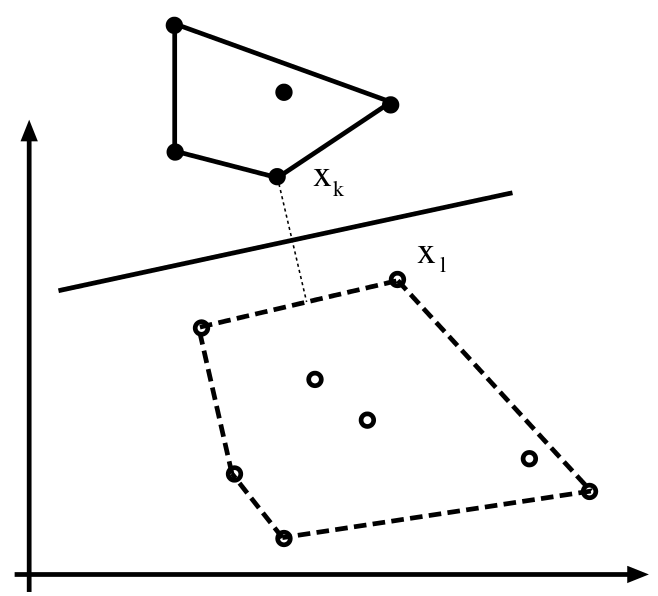
\includegraphics[width=0.75\textwidth]{figs/svm}
	\caption{Classification by a Support Vector Machine. The distance of the separating plane from both datasets is maximal. The figure was originally published in \cite{ponce2011cv}}
	\label{fig:svm}
	\end{figure}
	
	Assume that a set of pairs $\{\{\mathbf{x}_1, y_1\}, \{\mathbf{x}_2, y_2\}, ...\}$ where $x_\mathit{i}$ are features and $y_\mathit{i} \in \{-1, 1\}$ are labels is given. Further assume that points with different labels are two linearly-separable datasets as shown in the figure \ref{fig:svm}, where dots and circles are points with different labels. Then, there exist parameters \textbf{\textit{w}} and  \textit{b} which satisfies	
	\begin{equation}
	                        y_\mathit{i}\left(\mathbf{w}*\mathbf{x}_\mathit{i} + w\right) > 0                                                                                                                                                                                                                                                                                                                                                                                                                       
	                                                                                                                                                                                                                                                                                                                                                                                                                                               \end{equation}
	for every $\mathbf{x}_\mathit{i}$ or a data point. This equation specifies constraints on a plane (or a hyperplane in general) that separates the dataset. A Support Vector Machine finds parameters \textbf{\textit{w}} and  \textit{b} so as to maximise the distance of this plane from both datasets.
	
\section{Libraries}

	One of the advantages of object oriented programming is that it is easier to reuse once created code. There exists a variety of third party libraries for the C++ programming language. One of the biggest and the most widely used are the general purpose Boost libraries \cite{Boost}. In the fields of computer vision there are, among others, OpenCV \cite{OpenCV} and PointCloud Library \cite{PCL}. Easy to use and intuitive logging is provided by the Apache log4cxx \cite{log4cxx}.
	
	\subsection{PointCloud Library}
	Being nothing but a large scale open source project, it is a great processing tool for 2D images and 3D point clouds. Often abbreviated as PCL, it contains numerous state-of-the-art algorithms for feature detection, surface reconstruction, segmentation and many other subareas of computer vision. It is well documented and easy to use. Recently a machine learning library containing algorithms such as Support Vector Machine has been added. Some algorithms are multi-threaded thanks to the OpenMP library. A GPU module boosts some algorithms. Unfortunately the PCL is relatively new and its stability could be better. Currently available 1.7.0 version is going to be replaced by soon-to-be-announced 2.0 version with incompatible API.
	
	Every feature detector and descriptor used in this project comes from the PCL.
	
	\subsection{OpenCV}
	Considerably more mature, the OpenCV library is yet another great image processing library. A multitude of methods implemented in both C (OpenCV 1.x) and C++ (OpenCV 2.x) allows for production of fully functional image processing or computer vision application with this single library. There are many machine learning mechanisms as well. Among them one can find kMeans, Gaussian Mixture Model, Na\`ive Bayes or a Support Vector Machine. Some of the more demanding in terms of computational power are parallelized with Threading Building Blocks (TBB). A module exploiting powers of the nVidia's CUDA technology exists in order to enhance computation even more.
	
	In this paper OpenCV is used for input/output operations, image preprocessing. KMeans and SVM implementations are used as well.
	
	\subsection{Boost}
	Boost is a general purpose library. It contains more than 50 separate libraries, 12 of which were incorporated into the new C++11 standard. One of the most popular are libraries for smart pointers, multi-threading or meta-programming. Tagger3D uses only the functionality provided by the Boost.program\_options library. It enables convenient parsing of configuration files and command line arguments.
		
\section{Datasets}

	Multiple RGBD datasets were created. The purpose of authors of the vast majority of them were to provide a benchmark for tasks of tracking or instance-level object recognition. Others have small number of categories or very few examples in every category. Unfortunately, the most are not fit for the object classification problem.
	The RGB-D object dataset from the University of Washington \cite{dataset_washington} would be perfect, if not for the fact that it consists of video sequences. A technology like Kinect Fusion \cite{KinectFusion} makes it relatively easy to build a detailed 3D model (a point cloud or a mesh) from such data. The only problem is in the computational cost of this method and actions required to gather such data --- in a real setting a mobile robot would have to circle an object. Two datasets are used are for the purpose of this paper. The first one is the Berkeley 3D Object dataset \cite{B3DO} and the second one is a dataset compiled by Zhang \emph{et al} at the University of Tokyo \cite{zhangcategory}. The datasets are going to be abbreviated as B3DO and Tokyo datasets respectively


	\subsection{Berkeley 3D Object Dataset}
	\begin{figure}[!ht]
	\centering
	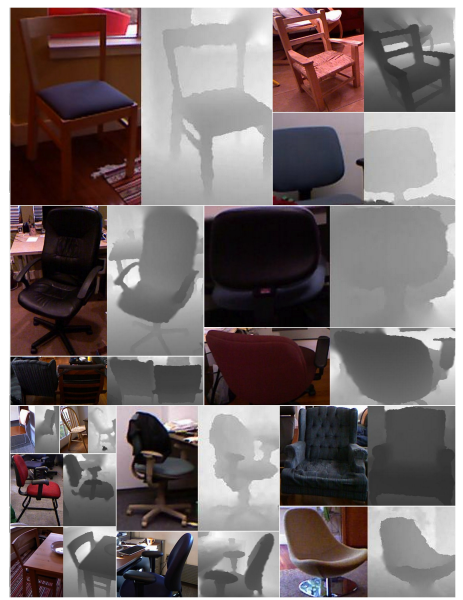
\includegraphics[width=0.5\textwidth]{figs/b3do_dataset}
	\caption{Berkeley 3D Object Dataset. The figure comes from \cite{B3DO}}
	\label{fig:b3do}
	\end{figure}
	
	The Berkeley 3D Object dataset was specifically designed for the purpose of object classification. It consists of cluttered images in indoor environment. There are around 50 classes with more than 20 examples in each of them. RGBD data is provided as pairs of images. There are 8 bit RGB jpeg pictures and 16 bit png files containing depth data in millimetres. Images are densely labelled --- for every pair of images there is an xml with annotations. Every annotation is comprised of a category label, bounding box coordinates and object's orientation.

	Before the B3DO database could be used it had to be preprocessed. Neither image segmentation nor object detection are addressed in this paper. Because of that the objects had to be extracted from the cluttered images.

	\subsection{The University of Tokyo Dataset}	
	\begin{figure}[!ht]
	\centering
	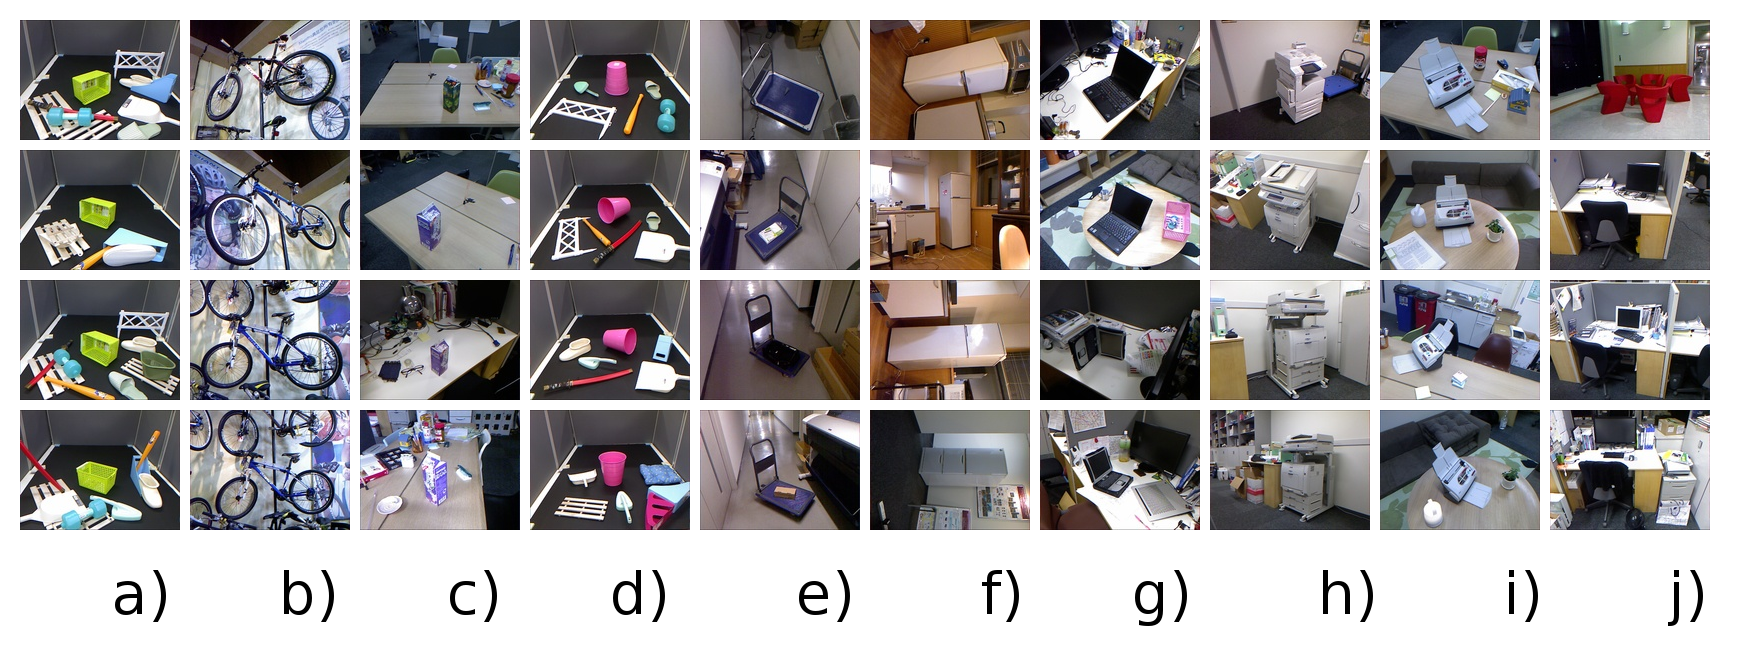
\includegraphics[width=1\textwidth]{figs/tokyo_horizontal}
	\caption{The Tokyo dataset: a) basket b) bicycle c) box d) bucket e) cart f) freezer g) notebook h) printer i) scanner j) scene}
	\label{fig:tokyo}
	\end{figure}
	
	The dataset compiled at the University of Tokyo is comprised of high quality images of objects in different settings. Factors such as viewpoint, object orientation, object's texture and environments are changing on different images. The aim of the authors of this dataset was slightly different - it was object detection and classification in casual images. There are 10 classes with varying amounts of per class examples. The database is available as two sets of files: 8 bit RGB jpeg files and csv files containing euclidean coordinates of every pixel in the corresponding colour image.


